% Provenance (never printed): cycle 2 "Questionner l'espace et le temps"
% (the globe, the continents and the oceans, reading a world map); see
% sources/book1/PROVENANCE.md. Book 1, grade 3, chapter 2.
\chapter{Le globe~: continents et océans}\label{ch:g3:continents-and-oceans}

Dans la classe de Lena, il y a un \omterm{def:g3:continents-and-oceans:globe}{globe} sur un pied. Lena ferme les yeux,
le fait tourner d'un doigt, puis l'arrête du bout du doigt. Elle ouvre les
yeux~: son doigt est sur du bleu, au milieu d'un \omterm{def:g2:water-on-earth:ocean}{océan}. Elle recommence~:
encore du bleu. La troisième fois, elle tombe sur du vert-jaune, quelque
part au milieu de l'Afrique.

Lena continue à jouer, et elle compte. Son doigt s'arrête bien plus souvent
sur la \omterm{def:g2:water-on-earth:ocean}{mer} que sur la terre. Pourquoi~? Et que sont toutes ces formes de
terre et d'eau qui défilent sous son doigt~?

\begin{omfigure}
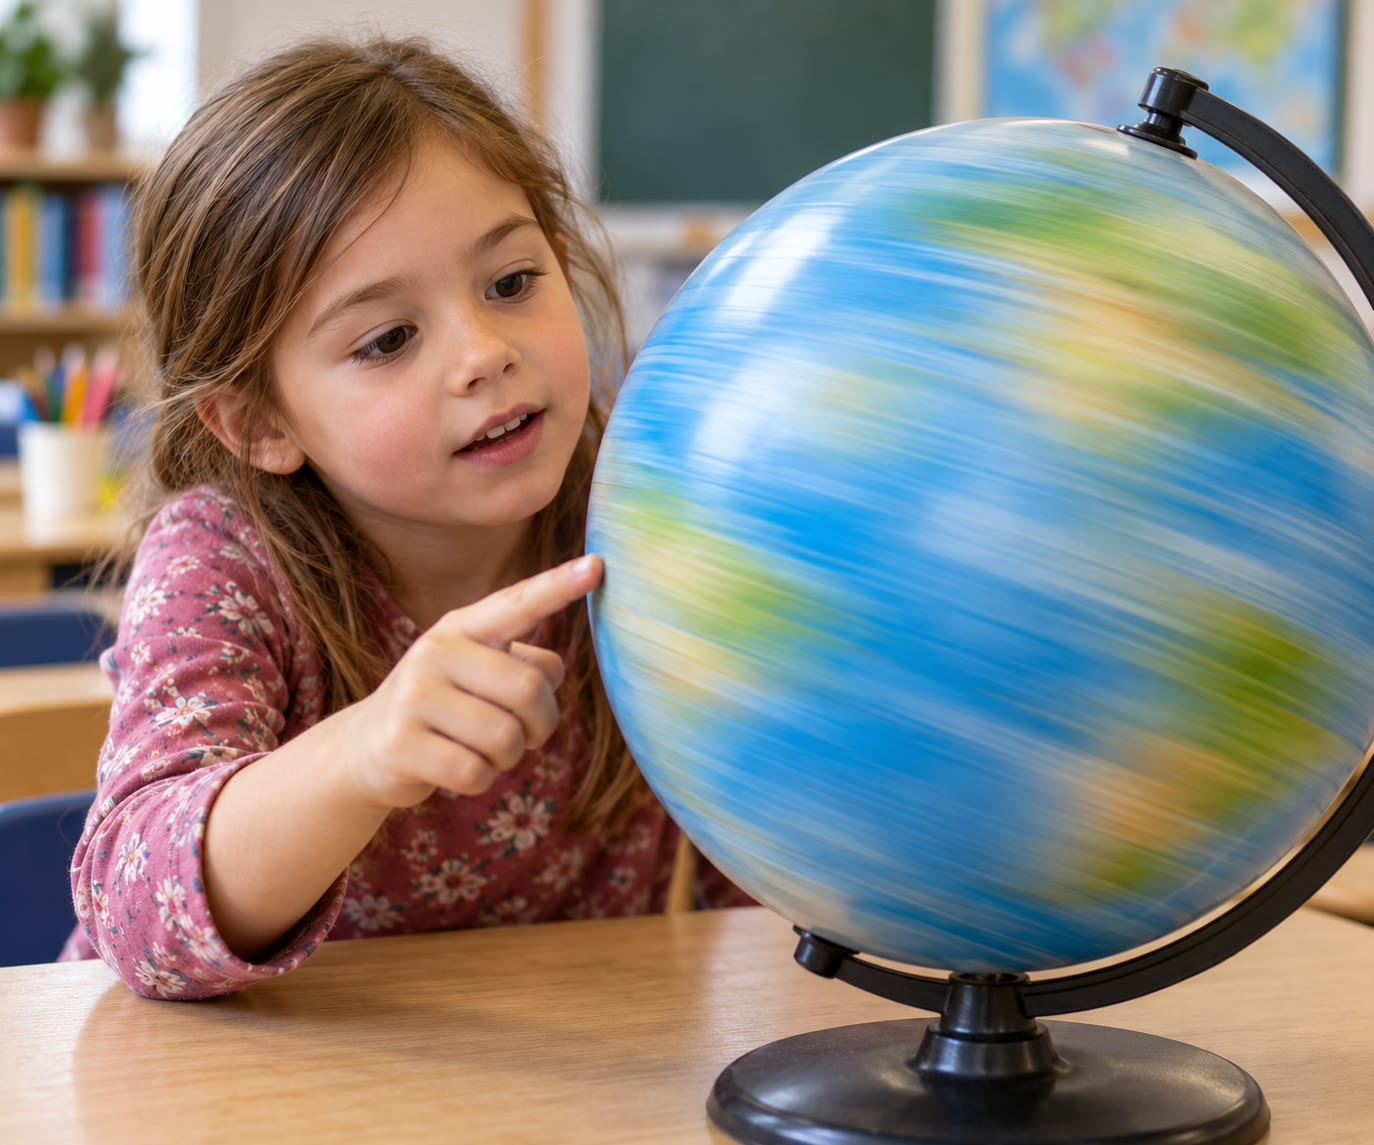
\includegraphics[width=0.6\linewidth]{images/book1/ai/g3-spinning-globe.jpg}

{\small Un \omterm{def:g3:continents-and-oceans:globe}{globe} qui tourne sur son pied~: la terre et la \omterm{def:g2:water-on-earth:ocean}{mer} défilent sous
le doigt.}
\end{omfigure}

\begin{recall}
La plus grande partie de la Terre est couverte d'\omterm{def:g2:water-on-earth:salt-fresh}{eau salée}~: environ
71 carrés sur 100 sur la grille du \cref{ch:g2:water-on-earth}. Un \omterm{def:g2:water-on-earth:ocean}{océan}
est une très grande étendue d'\omterm{def:g2:water-on-earth:salt-fresh}{eau salée} entre les terres~; une \omterm{def:g2:water-on-earth:ocean}{mer} est une
étendue plus petite, au bord d'un \omterm{def:g2:water-on-earth:ocean}{océan}. Une \omterm{def:g2:drawing-to-map:map}{carte} est le dessin d'un lieu
vu d'en haut, en plus petit (\cref{ch:g2:drawing-to-map}). Les livres de
physique racontent comment la Terre tourne sur elle-même une fois par
jour, ce qui nous donne le jour et la nuit.
\end{recall}

\section{Le globe, un petit modèle de la Terre ronde}

La Terre est ronde, comme un très gros ballon. Depuis le sol, nous ne
voyons pas sa forme, car elle est bien trop grande~: où que nous soyons, le
sol paraît plat. Mais les astronautes qui sont allés loin de la Terre l'ont
vue tout entière, une boule bleue et ronde dans le ciel noir (la
photographie du début du \cref{ch:g2:water-on-earth}).

Pour voir toute la Terre dans une salle de classe, nous la faisons toute petite.

\begin{definition}[Globe]\label{def:g3:continents-and-oceans:globe}
Un \emph{globe}\index{globe} est un modèle de la Terre~: une boule sur
laquelle les terres et les \omterm{def:g2:water-on-earth:ocean}{océans} sont dessinés avec les mêmes formes que
sur la vraie Terre, mais en beaucoup plus petit.
\end{definition}

Le \omterm{def:g3:continents-and-oceans:globe}{globe} est la meilleure image de la Terre, parce qu'il a la bonne
forme~: il est rond. Mais, comme pour la vraie Terre, nous n'en voyons
jamais qu'une moitié à la fois. Pour voir l'autre moitié, nous le faisons
tourner.

\begin{omfigure}
\begin{tikzpicture}
\begin{axis}[name=atl, hide axis, axis equal image, scale only axis,
    width=6.2cm, xmin=-1.05, xmax=1.05, ymin=-1.05, ymax=1.05, clip=false]
  \fill[omSea] (axis cs:0,0) circle[radius=1];
  \addplot[fill=omHypsLandA!85!black, draw=black!45, line width=0.2pt]
    table {figdata/out/grade-3-globe-atlantic-land.dat};
  \addplot[black!60, dashed, line width=0.5pt]
    table {figdata/out/grade-3-globe-atlantic-equator.dat};
  \addplot[only marks, mark=*, mark size=1.4pt, black]
    table[x=x, y=y] {figdata/out/grade-3-globe-atlantic-poles.dat};
  \node[font=\scriptsize, anchor=center, align=center, fill=white, fill opacity=0.7, text opacity=1, inner sep=1pt, rounded corners=1pt] at (axis cs:-0.683,0.636) {Amérique\\du Nord};
  \node[font=\scriptsize, anchor=center, align=center, fill=white, fill opacity=0.7, text opacity=1, inner sep=1pt, rounded corners=1pt] at (axis cs:-0.561,-0.408) {Amérique\\du Sud};
  \node[font=\scriptsize, anchor=center, align=center, fill=white, fill opacity=0.7, text opacity=1, inner sep=1pt, rounded corners=1pt] at (axis cs:0.396,0.639) {Europe};
  \node[font=\scriptsize, anchor=center, align=center, fill=white, fill opacity=0.7, text opacity=1, inner sep=1pt, rounded corners=1pt] at (axis cs:0.704,-0.098) {Afrique};
  \node[font=\scriptsize, anchor=center, align=center, fill=white, fill opacity=0.7, text opacity=1, inner sep=1pt, rounded corners=1pt] at (axis cs:-0.209,0.128) {Océan\\Atlantique};
  \draw[black!70, line width=0.8pt] (axis cs:0,0) circle[radius=1];
  \node[font=\scriptsize, anchor=south] at (axis cs:0,0.97) {pôle Nord};
\end{axis}
\begin{axis}[at={(atl.east)}, anchor=west, xshift=0.6cm, hide axis,
    axis equal image, scale only axis,
    width=6.2cm, xmin=-1.05, xmax=1.05, ymin=-1.05, ymax=1.05, clip=false]
  \fill[omSea] (axis cs:0,0) circle[radius=1];
  \addplot[fill=omHypsLandA!85!black, draw=black!45, line width=0.2pt]
    table {figdata/out/grade-3-globe-pacific-land.dat};
  \addplot[black!60, dashed, line width=0.5pt]
    table {figdata/out/grade-3-globe-pacific-equator.dat};
  \node[font=\scriptsize, anchor=center, align=center, fill=white, fill opacity=0.7, text opacity=1, inner sep=1pt, rounded corners=1pt] at (axis cs:-0.754,-0.391) {Australie};
  \node[font=\scriptsize, anchor=center, align=center, fill=white, fill opacity=0.7, text opacity=1, inner sep=1pt, rounded corners=1pt] at (axis cs:0.258,0.087) {Océan\\Pacifique};
  \draw[black!70, line width=0.8pt] (axis cs:0,0) circle[radius=1];
\end{axis}
\end{tikzpicture}

{\small Le \omterm{def:g3:continents-and-oceans:globe}{globe} vu de deux côtés. À gauche~: le côté de l'\omterm{def:g2:water-on-earth:ocean}{océan}
Atlantique, avec les Amériques, l'Europe et l'Afrique. À droite~: l'autre
côté, l'\omterm{def:g2:water-on-earth:ocean}{océan} Pacifique, avec l'Australie à son bord. La ligne en tirets
est l'\omterm{def:g3:continents-and-oceans:equator}{équateur}. Contours des côtes~: Natural Earth (domaine public).}
\label{fig:g3:continents-and-oceans:globes}
% ledger: data:ne-land
\end{omfigure}

\begin{remark}[Deux moitiés très différentes]\label{rem:g3:continents-and-oceans:halves}
Regarde les deux images. À gauche, les terres couvrent environ 4 parties
de l'image sur 10. À droite, environ 1 partie sur 10 seulement~: le côté
Pacifique de la Terre est presque entièrement couvert d'eau. Si le doigt
de Lena s'arrête de ce côté du \omterm{def:g3:continents-and-oceans:globe}{globe}, il tombera presque toujours sur la
\omterm{def:g2:water-on-earth:ocean}{mer}.
\end{remark}

\section{L'équateur, les pôles et les deux hémisphères}

Un \omterm{def:g3:continents-and-oceans:globe}{globe} tourne autour d'une tige qui le traverse de haut en bas. La vraie
Terre n'a pas de tige, mais elle tourne elle aussi autour d'une ligne qui
passe par son milieu. Les deux endroits où cette ligne sort de la Terre
portent un nom.

\begin{definition}[Pôle]\label{def:g3:continents-and-oceans:poles}
Le \emph{pôle Nord}\index{pole Nord@pôle Nord} et le
\emph{pôle Sud}\index{pole Sud@pôle Sud} sont les deux points tout en haut
et tout en bas de la Terre, là où sort la ligne autour de laquelle la Terre
tourne. Chacun d'eux est un \emph{pôle}\index{pole@pôle}. Sur un \omterm{def:g3:continents-and-oceans:globe}{globe}, le
pôle Nord est en haut.
\end{definition}

\begin{definition}[Équateur et hémisphère]\label{def:g3:continents-and-oceans:equator}
L'\emph{équateur}\index{equateur@équateur} est une ligne imaginaire tracée
tout autour de la Terre, exactement à mi-chemin entre le \omterm{def:g3:continents-and-oceans:poles}{pôle Nord} et le
\omterm{def:g3:continents-and-oceans:poles}{pôle Sud}. Il coupe la Terre en deux moitiés, appelées chacune un
\emph{hémisphère}\index{hemisphere@hémisphère}~:
l'\emph{hémisphère nord}\index{hemisphere nord@hémisphère nord}, du côté du
\omterm{def:g3:continents-and-oceans:poles}{pôle Nord}, et l'\emph{hémisphère sud}\index{hemisphere sud@hémisphère sud},
du côté du \omterm{def:g3:continents-and-oceans:poles}{pôle Sud}.
\end{definition}

L'\omterm{def:g3:continents-and-oceans:equator}{équateur} n'est pas peint sur le sol~: personne ne peut le voir sur une
plage ou dans une forêt. On le dessine sur les \omterm{def:g3:continents-and-oceans:globe}{globes} et sur les \omterm{def:g2:drawing-to-map:map}{cartes}
pour nous aider à nous repérer.

\begin{omfigure}
\begin{tikzpicture}[font=\small]
  % globe outline
  \fill[omSea!70] (0,0) circle (2.2);
  % northern hemisphere tinted
  \begin{scope}
    \clip (0,0) circle (2.2);
    \fill[yellow!25, opacity=0.8] (-2.3,0) -- (-2.3,2.3) -- (2.3,2.3) -- (2.3,0)
      arc[start angle=0, end angle=-180, x radius=2.3, y radius=0.45] -- cycle;
  \end{scope}
  \draw[black!70, line width=0.8pt] (0,0) circle (2.2);
  % equator: front half solid, back half dashed
  \draw[red!70!black, line width=1.2pt] (-2.2,0) arc[start angle=180, end angle=360, x radius=2.2, y radius=0.4];
  \draw[red!70!black, line width=0.8pt, dashed] (2.2,0) arc[start angle=0, end angle=180, x radius=2.2, y radius=0.4];
  % axis and poles
  \draw[black!60, line width=0.6pt] (0,2.2) -- (0,2.75);
  \draw[black!60, line width=0.6pt] (0,-2.2) -- (0,-2.75);
  \draw[black!60, line width=0.6pt, dotted] (0,2.2) -- (0,-2.2);
  \fill (0,2.2) circle (2.2pt);
  \fill (0,-2.2) circle (2.2pt);
  \node[anchor=west] at (0.15,2.6) {pôle Nord};
  \node[anchor=west] at (0.15,-2.6) {pôle Sud};
  % labels
  \node[anchor=west] at (2.6,0) {équateur};
  \draw[black!60] (2.55,0) -- (2.05,-0.15);
  \node[anchor=west, align=left] at (2.6,1.4) {hémisphère\\nord};
  \draw[black!60] (2.55,1.4) -- (1.5,1.2);
  \node[anchor=west, align=left] at (2.6,-1.4) {hémisphère\\sud};
  \draw[black!60] (2.55,-1.4) -- (1.5,-1.2);
\end{tikzpicture}

{\small L'\omterm{def:g3:continents-and-oceans:equator}{équateur} coupe la Terre en deux \omterm{def:g3:continents-and-oceans:equator}{hémisphères}. L'\omterm{def:g3:continents-and-oceans:equator}{hémisphère nord}
(teinté) est du côté du \omterm{def:g3:continents-and-oceans:poles}{pôle Nord}, l'\omterm{def:g3:continents-and-oceans:equator}{hémisphère sud} du côté du \omterm{def:g3:continents-and-oceans:poles}{pôle Sud}.}
\label{fig:g3:continents-and-oceans:hemispheres}
\end{omfigure}

\begin{example}[Chaud près de l'équateur, froid près des pôles]\label{ex:g3:continents-and-oceans:hot-cold}
Les terres proches de l'\omterm{def:g3:continents-and-oceans:equator}{équateur} sont chaudes toute l'année~: c'est là que
poussent les grandes forêts tropicales humides. Les terres proches des
\omterm{def:g3:continents-and-oceans:poles}{pôles} sont froides toute l'année, et une grande partie est couverte de
glace. Tu apprendras dans une année suivante pourquoi il en est ainsi~;
pour l'instant, retiens~: plus on est près d'un \omterm{def:g3:continents-and-oceans:poles}{pôle}, plus il fait froid.
\end{example}

\section{Sept continents et cinq océans}

Sur un \omterm{def:g3:continents-and-oceans:globe}{globe}, les terres ne sont pas éparpillées partout en petits
morceaux. Elles sont presque toutes rassemblées en quelques très grandes
masses.

\begin{definition}[Continent]\label{def:g3:continents-and-oceans:continent}
Un \emph{continent}\index{continent} est l'une des très grandes masses de
terre de la Terre, avec les îles qui en sont proches.
\end{definition}

On compte le plus souvent sept \omterm{def:g3:continents-and-oceans:continent}{continents}. Du plus grand au plus petit, ce
sont~: l'Asie, l'Afrique, l'Amérique du Nord, l'Amérique du Sud,
l'Antarctique, l'Europe et l'Australie.
% ledger: natgeo:seven-continents

\begin{center}\small
\begin{tabular}{rlll}
\hline
Rang & \omterm{def:g3:continents-and-oceans:continent}{Continent} & \omterm{def:g3:continents-and-oceans:equator}{Hémisphère} & Un mot sur lui \\
\hline
1 & Asie & surtout nord & le plus grand \\
2 & Afrique & les deux & l'\omterm{def:g3:continents-and-oceans:equator}{équateur} passe en son milieu \\
3 & Amérique du Nord & nord & s'étend très loin vers le nord \\
4 & Amérique du Sud & surtout sud & l'\omterm{def:g3:continents-and-oceans:equator}{équateur} traverse son nord \\
5 & Antarctique & sud & autour du \omterm{def:g3:continents-and-oceans:poles}{pôle Sud}, sous la glace \\
6 & Europe & nord & soudée à l'Asie sur son côté est \\
7 & Australie & sud & le plus petit \\
\hline
\end{tabular}
\end{center}

\begin{remark}[Où s'arrête un continent~?]\label{rem:g3:continents-and-oceans:where}
Certains \omterm{def:g3:continents-and-oceans:continent}{continents} sont entourés par la \omterm{def:g2:water-on-earth:ocean}{mer} de tous les côtés, comme
l'Australie ou l'Antarctique. D'autres se touchent~: l'Europe et l'Asie ne
forment qu'une seule masse de terre, et ce sont les gens qui ont choisi
où tracer la limite entre elles. C'est pourquoi certains comptent six
\omterm{def:g3:continents-and-oceans:continent}{continents}, ou même moins.
\end{remark}

Entre les \omterm{def:g3:continents-and-oceans:continent}{continents} s'étendent les \omterm{def:g2:water-on-earth:ocean}{océans}. Il y en a cinq. Le plus grand
est l'\emph{\omterm{def:g2:water-on-earth:ocean}{océan} Pacifique}~; viennent ensuite l'\emph{\omterm{def:g2:water-on-earth:ocean}{océan} Atlantique},
l'\emph{\omterm{def:g2:water-on-earth:ocean}{océan} Indien}, l'\emph{\omterm{def:g2:water-on-earth:ocean}{océan} Austral} autour de l'Antarctique, et
le plus petit, l'\emph{\omterm{def:g2:water-on-earth:ocean}{océan} Arctique} autour du \omterm{def:g3:continents-and-oceans:poles}{pôle Nord}. Pendant
longtemps, on n'en comptait que quatre~; aujourd'hui, la plupart des pays
comptent l'\omterm{def:g2:water-on-earth:ocean}{océan} Austral comme le cinquième.
% ledger: nos:five-oceans, nos:pacific-largest, oer:arctic-smallest

\begin{example}[Quelle est la taille du Pacifique~?]\label{ex:g3:continents-and-oceans:pacific}
L'\omterm{def:g2:water-on-earth:ocean}{océan} Pacifique est si grand que tous les \omterm{def:g3:continents-and-oceans:continent}{continents} réunis pourraient
y tenir. Il contient plus de la moitié de toute l'eau des \omterm{def:g2:water-on-earth:ocean}{océans} de la
Terre. C'est pourquoi le \omterm{def:g3:continents-and-oceans:globe}{globe} de droite, dans la première section de ce
chapitre, paraît presque tout bleu.
% ledger: nos:pacific-largest
\end{example}

\begin{method}[Nommer l'océan entre deux continents]\label{met:g3:continents-and-oceans:between}
Pour trouver quel \omterm{def:g2:water-on-earth:ocean}{océan} s'étend entre deux \omterm{def:g3:continents-and-oceans:continent}{continents}, pose un doigt sur
chacun d'eux sur le \omterm{def:g3:continents-and-oceans:globe}{globe}, et tourne le \omterm{def:g3:continents-and-oceans:globe}{globe} de façon à voir les deux.
L'\omterm{def:g2:water-on-earth:ocean}{océan} que ton œil traverse pour aller d'un doigt à l'autre est celui qui
les sépare. Sur un \omterm{def:g3:continents-and-oceans:globe}{globe}, il y a souvent deux chemins possibles~: prends
le plus court.
\end{method}

\begin{example}[L'Afrique et l'Australie]\label{ex:g3:continents-and-oceans:africa-australia}
En allant de l'Afrique vers l'est jusqu'à l'Australie, nous traversons
l'\omterm{def:g2:water-on-earth:ocean}{océan} Indien. En allant de l'Europe vers l'ouest jusqu'à l'Amérique du
Nord, nous traversons l'\omterm{def:g2:water-on-earth:ocean}{océan} Atlantique. En allant de l'Asie vers l'est
jusqu'à l'Amérique du Nord, nous traversons l'\omterm{def:g2:water-on-earth:ocean}{océan} Pacifique.
\end{example}

\section{Un planisphère est un globe aplati}

Un \omterm{def:g3:continents-and-oceans:globe}{globe} est rond~: il n'est pas facile à transporter, et nous ne pouvons
jamais le voir en entier d'un coup. Une \omterm{def:g2:drawing-to-map:map}{carte} sur une feuille de papier
montre toute la Terre d'un seul regard.

\begin{definition}[Planisphère]\label{def:g3:continents-and-oceans:world-map}
Un \emph{planisphère}\index{planisphere@planisphère} est une \omterm{def:g2:drawing-to-map:map}{carte} de toute
la Terre dessinée à plat, sur une feuille de papier ou sur un écran, avec
tous les \omterm{def:g3:continents-and-oceans:continent}{continents} et tous les \omterm{def:g2:water-on-earth:ocean}{océans} sur une seule image.
\end{definition}

\begin{omfigure}
\begin{tikzpicture}
\begin{axis}[ommap, width=\linewidth, xtick=\empty, ytick={0},
    yticklabels={équateur}, grid=none, clip=true]
  \addplot[fill=omHypsLandA!85!black, draw=black!45, line width=0.2pt]
    table {figdata/out/shared-geo-land.dat};
  \draw[black!60, dashed, line width=0.5pt] (axis cs:-180,0) -- (axis cs:180,0);
  \begin{scope}[every node/.style={font=\scriptsize, align=center}]
    \node at (axis cs:-102,47) {Amérique\\du Nord};
    \node at (axis cs:-60,-12) {Amérique\\du Sud};
    \node at (axis cs:17,52) {Europe};
    \node at (axis cs:20,6) {Afrique};
    \node at (axis cs:92,48) {Asie};
    \node at (axis cs:134,-24) {Australie};
    \node at (axis cs:40,-80) {Antarctique};
  \end{scope}
  \begin{scope}[every node/.style={font=\scriptsize\itshape, align=center, text=omSea!35!black}]
    \node at (axis cs:-145,8) {Océan\\Pacifique};
    \node at (axis cs:165,12) {Océan\\Pacifique};
    \node at (axis cs:-38,22) {Océan\\Atlantique};
    \node at (axis cs:-15,-25) {Océan\\Atlantique};
    \node at (axis cs:78,-22) {Océan\\Indien};
    \node at (axis cs:-115,-57) {Océan Austral};
    \node at (axis cs:-150,79) {Océan Arctique};
  \end{scope}
\end{axis}
\end{tikzpicture}

{\small Un \omterm{def:g3:continents-and-oceans:world-map}{planisphère}. Le \omterm{def:g3:continents-and-oceans:globe}{globe} a été coupé le long d'une ligne passant
par le milieu de l'\omterm{def:g2:water-on-earth:ocean}{océan} Pacifique, puis étalé à plat~: le Pacifique
apparaît deux fois, au bord gauche et au bord droit. L'Antarctique, un
\omterm{def:g3:continents-and-oceans:continent}{continent} rond autour du \omterm{def:g3:continents-and-oceans:poles}{pôle Sud}, est étiré en une longue bande tout en
bas. Contours des côtes~: Natural Earth (domaine public).}
\label{fig:g3:continents-and-oceans:world-map}
% ledger: data:ne-land
\end{omfigure}

Mais il y a une difficulté. Essaie d'aplatir la peau d'une orange sur une
table~: elle ne peut pas rester à plat sans se déchirer ou s'étirer. Il
arrive la même chose à la surface du \omterm{def:g3:continents-and-oceans:globe}{globe} quand on la dessine à plat.
Tout \omterm{def:g3:continents-and-oceans:world-map}{planisphère} déchire le \omterm{def:g3:continents-and-oceans:globe}{globe} quelque part, ou bien étire certains
endroits et en écrase d'autres.

\begin{omfigure}
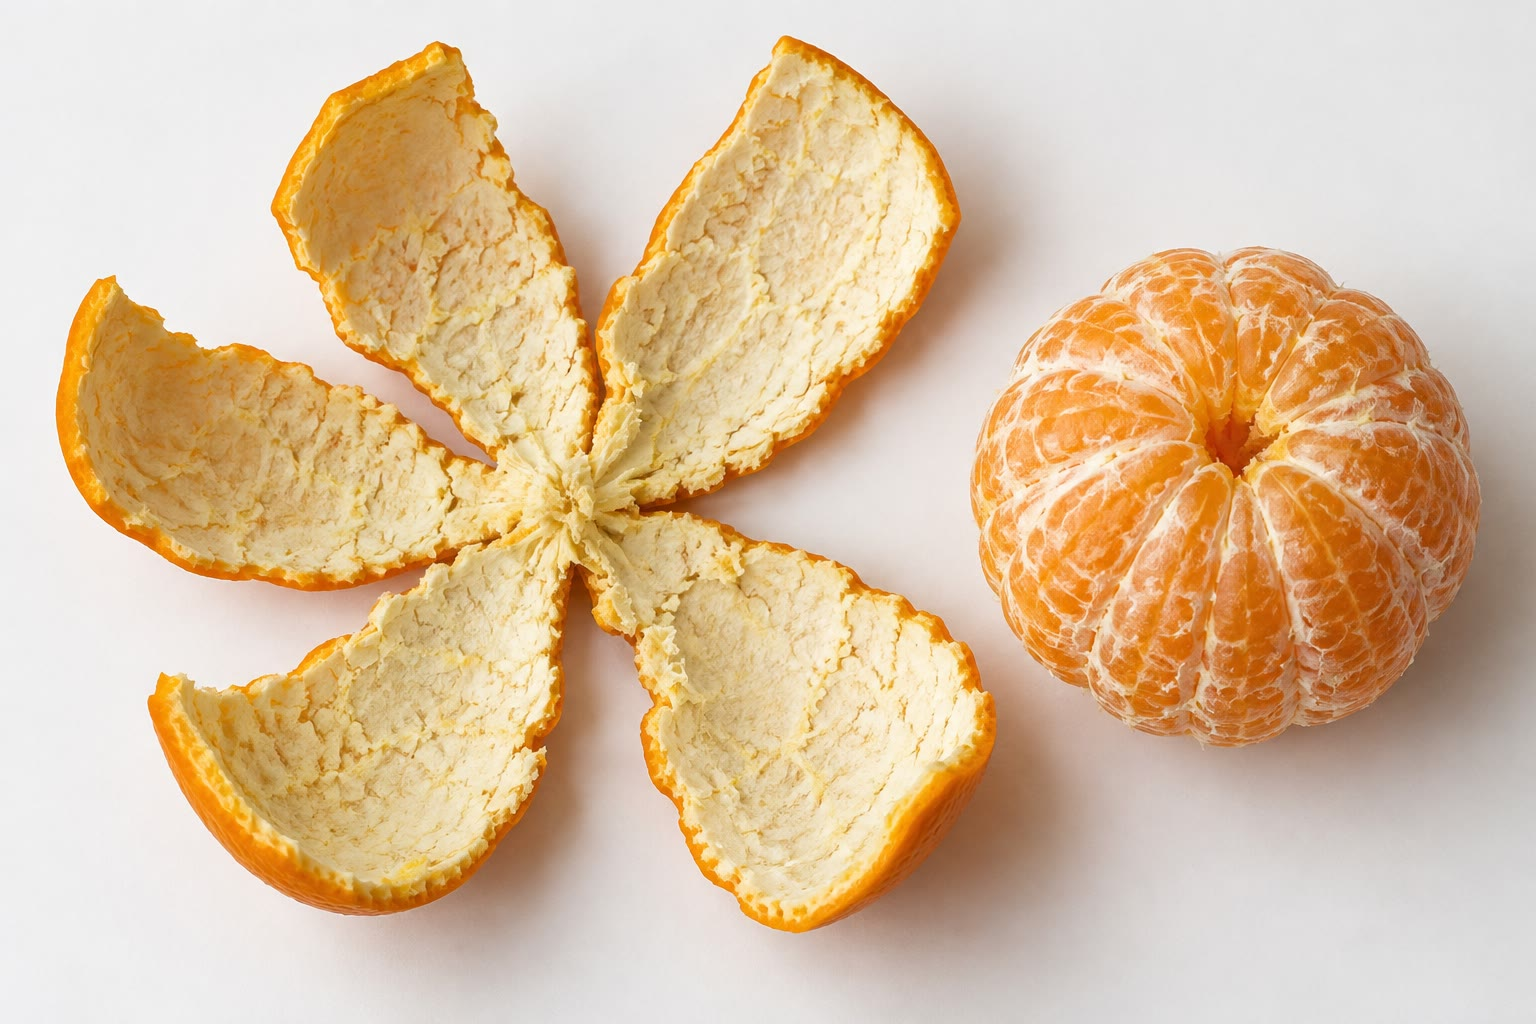
\includegraphics[width=0.4\linewidth]{images/book1/ai/g3-orange-peel.jpg}

{\small La peau d'une orange ne peut pas rester à plat sans se déchirer.}
\end{omfigure}

\begin{remark}[La carte et le globe ne sont pas d'accord]\label{rem:g3:continents-and-oceans:disagree}
Sur ce \omterm{def:g3:continents-and-oceans:world-map}{planisphère}, l'Antarctique paraît être l'un des plus grands
\omterm{def:g3:continents-and-oceans:continent}{continents}, étiré tout le long du bord inférieur. Sur le \omterm{def:g3:continents-and-oceans:globe}{globe}, c'est une
masse de terre ronde, plus petite que l'Amérique du Sud. Près des \omterm{def:g3:continents-and-oceans:poles}{pôles},
une \omterm{def:g2:drawing-to-map:map}{carte} plate étire beaucoup les terres. Près de l'\omterm{def:g3:continents-and-oceans:equator}{équateur}, elle les
étire très peu. Quand tu veux comparer la taille de deux endroits loin de
l'\omterm{def:g3:continents-and-oceans:equator}{équateur}, c'est le \omterm{def:g3:continents-and-oceans:globe}{globe} qui dit vrai.
\end{remark}

\begin{method}[Lire un planisphère]\label{met:g3:continents-and-oceans:reading}
Sur un \omterm{def:g3:continents-and-oceans:world-map}{planisphère} comme celui-ci~:
\begin{enumerate}
  \item le nord est en haut, le sud en bas~; le \omterm{def:g3:continents-and-oceans:poles}{pôle Nord} est tout le bord
        supérieur et le \omterm{def:g3:continents-and-oceans:poles}{pôle Sud} tout le bord inférieur~;
  \item l'\omterm{def:g3:continents-and-oceans:equator}{équateur} est la ligne qui traverse le milieu~: tout ce qui est
        au-dessus est dans l'\omterm{def:g3:continents-and-oceans:equator}{hémisphère nord}, tout ce qui est en dessous
        dans l'\omterm{def:g3:continents-and-oceans:equator}{hémisphère sud}~;
  \item les bords gauche et droit sont la même ligne sur le \omterm{def:g3:continents-and-oceans:globe}{globe}~: un
        bateau qui sort par le bord droit revient par le bord gauche.
\end{enumerate}
\end{method}

\section{Exercices}

\begin{exercise}[$\star$]\label{exo:g3:continents-and-oceans:1}
Nomme les sept \omterm{def:g3:continents-and-oceans:continent}{continents}. Lequel est le plus grand~? Lequel est le plus petit~?
\end{exercise}

\begin{exercise}[$\star$]\label{exo:g3:continents-and-oceans:2}
Nomme les cinq \omterm{def:g2:water-on-earth:ocean}{océans}. Lequel est le plus grand~? Lequel est le plus petit~?
\end{exercise}

\begin{exercise}[$\star$]\label{exo:g3:continents-and-oceans:3}
Recopie et complète avec «~le \omterm{def:g3:continents-and-oceans:poles}{pôle Nord}~», «~le \omterm{def:g3:continents-and-oceans:poles}{pôle Sud}~» ou
«~l'\omterm{def:g3:continents-and-oceans:equator}{équateur}~»~: \dots{} est en haut d'un \omterm{def:g3:continents-and-oceans:globe}{globe}~; \dots{} est en bas~;
\dots{} fait tout le tour du milieu.
\end{exercise}

\begin{exercise}[$\star$]\label{exo:g3:continents-and-oceans:4}
\omterm{def:g3:continents-and-oceans:equator}{Hémisphère nord} ou \omterm{def:g3:continents-and-oceans:equator}{hémisphère sud}~? L'Europe~; l'Australie~;
l'Antarctique~; l'Amérique du Nord.
\end{exercise}

\begin{exercise}[$\star$]\label{exo:g3:continents-and-oceans:5}
Quel \omterm{def:g2:water-on-earth:ocean}{océan} entoure le \omterm{def:g3:continents-and-oceans:poles}{pôle Nord}~? Quel \omterm{def:g2:water-on-earth:ocean}{océan} entoure l'Antarctique~?
\end{exercise}

\begin{exercise}[$\star\star$]\label{exo:g3:continents-and-oceans:6}
Quel \omterm{def:g2:water-on-earth:ocean}{océan} traverses-tu pour aller de l'Afrique à l'Amérique du Sud~? De
l'Australie à l'Amérique du Sud, en allant vers l'est~? De l'Afrique à
l'Australie~?
\end{exercise}

\begin{exercise}[$\star\star$]\label{exo:g3:continents-and-oceans:7}
Sam vit dans un pays où il fait chaud toute l'année. Bo vit dans une base
scientifique où il gèle toute l'année. L'un d'eux vit près de l'\omterm{def:g3:continents-and-oceans:equator}{équateur},
l'autre près d'un \omterm{def:g3:continents-and-oceans:poles}{pôle}. Qui vit où~?
\end{exercise}

\begin{exercise}[$\star\star$]\label{exo:g3:continents-and-oceans:8}
Lena fait tourner le \omterm{def:g3:continents-and-oceans:globe}{globe} 10 fois. Son doigt tombe sur la \omterm{def:g2:water-on-earth:ocean}{mer} 7 fois.
Combien de fois tombe-t-il sur la terre~? Est-ce ce à quoi tu t'attendais~?
Pourquoi~?
\end{exercise}

\begin{exercise}[$\star\star$]\label{exo:g3:continents-and-oceans:9}
Sur le \omterm{def:g3:continents-and-oceans:world-map}{planisphère} de la page~\pageref{fig:g3:continents-and-oceans:world-map},
l'\omterm{def:g2:water-on-earth:ocean}{océan} Pacifique apparaît deux fois. Pourquoi~? La vraie Terre a-t-elle
deux \omterm{def:g2:water-on-earth:ocean}{océans} Pacifiques~?
\end{exercise}

\begin{exercise}[$\star\star\star$]\label{exo:g3:continents-and-oceans:10}
Tom dit~: «~Sur le \omterm{def:g3:continents-and-oceans:world-map}{planisphère}, l'Antarctique est plus long que l'Asie,
donc l'Antarctique est le plus grand \omterm{def:g3:continents-and-oceans:continent}{continent}.~» Tom a-t-il raison~?
Utilise la liste des \omterm{def:g3:continents-and-oceans:continent}{continents} du plus grand au plus petit, et explique
pourquoi le \omterm{def:g3:continents-and-oceans:world-map}{planisphère} le trompe.
\end{exercise}
